\documentclass{article}
% translate with >> pdflatex -shell-escape <file>

% This file is used as unit test for pgfplots, copyright by Christian Feuersaenger.
% 
% See
%   http://pgfplots.sourceforge.net/pgfplots.pdf
% for pgfplots.
%
% Any required input files (for <plot table> or <plot file> or the table package) can be downloaded
% at
% http://www.ctan.org/tex-archive/graphics/pgf/contrib/pgfplots/doc/latex/
% and
% http://www.ctan.org/tex-archive/graphics/pgf/contrib/pgfplots/doc/latex/plotdata/

\usepackage{pgfplots}
\pgfplotsset{compat=1.4}

\usepgfplotslibrary{patchplots}
\pagestyle{empty}

\begin{document}
\pgfplotsset{show nodes/.style={nodes near coords=\coordindex,nodes near coords align={center}}}
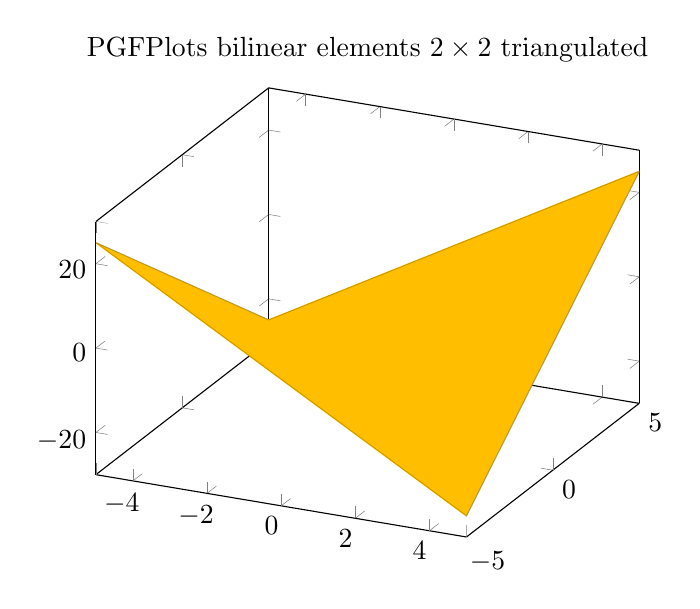
\begin{tikzpicture}
			\begin{axis}[title=bilinear,title={PGFPlots bilinear elements $2 \times 2$ triangulated}]
			\addplot3[surf,patch type=bilinear,samples=2] {x*y};
			\end{axis}
		\end{tikzpicture}
\end{document}
